% Subsection about followers

Dans le schéma de la Figure \ref{fig2:schematics}, les filtres passifs sont isolés les uns des autres grâce à des \emph{amplificateurs}, placés dans des montages suiveurs. Pour réaliser ces montages, nous allons utiliser un chip, le LM358N, représenté sur la Figure \ref{fig:LM358N_pic}, qui contient en fait deux amplificateurs. Ce chip a aussi une encoche pour donner l'information sur le sens de branchement. Chaque patte/pin du circuit a une fonction différente, comme renseigné sur la Figure \ref{fig:LM358N_pins}. Par exemple, la patte $V_{cc-}$ (pin 4) doit être connectée à une alimentation de $-15 V$ et la patte $V_{cc+}$ (pin 8) doit être connectée à une alimentation de $+15 V$. Les pins 1 à 3 sont les entrées/sortie du premier amplificateur, les pins 5 à 7 sont celles du second.

\begin{minipage}[c]{.49\textwidth}
	\centering
	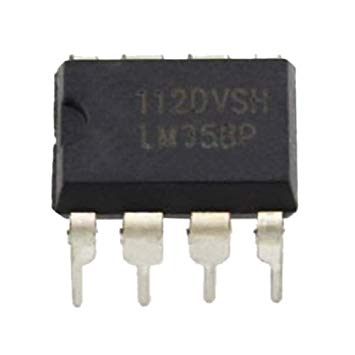
\includegraphics[width=0.6\textwidth]{figures/LM358N_picture.jpg}
	\captionof{figure}{Photo de du chip LM358N.}
	\label{fig:LM358N_pic}
\end{minipage}
\hfill
\begin{minipage}[c]{.49\textwidth}
	\centering
	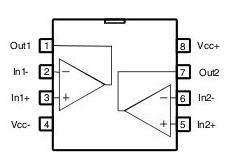
\includegraphics[width=\textwidth]{figures/LM358N_connections.jpg}
	\captionof{figure}{Nom des pattes du chip LM358N.}
	\label{fig:LM358N_pins}
\end{minipage}
\vspace{1cm}

Un \emph{montage suiveur} consiste à connecter la sortie d'un amplificateur à son entrée négative ($IN-$). La sortie va alors \emph{suivre} l'entrée positive ($IN+$). Ce montage permet d'isoler ce qui suit l'amplificateur de ce qui le précède, car l'amplificateur a une haute impédance d'entrée et une très faible impédance de sortie.